% This file was converted to LaTeX by Writer2LaTeX ver. 0.4b
% see http://www.hj-gym.dk/~hj/writer2latex for more info
\documentclass[12pt,twoside]{article}
\usepackage[ascii]{inputenc}
\usepackage[T1]{fontenc}
\usepackage[english]{babel}
\usepackage{amsmath,amssymb,amsfonts,textcomp}
\usepackage{color}
\usepackage{calc}
\usepackage{hyperref}
\usepackage{graphicx}
\hypersetup{colorlinks=true, linkcolor=blue, filecolor=blue, pagecolor=blue, urlcolor=blue}
% Text styles
\newcommand\textstyleInternetlink[1]{\textcolor{blue}{#1}}
% Outline numbering
\setcounter{secnumdepth}{0}
% List styles
\newcounter{saveenum}
\newcommand\liststyleWWviiiNumii{%
\renewcommand\labelitemi{[F0B7?]}
\renewcommand\labelitemii{o}
\renewcommand\labelitemiii{[F0A7?]}
\renewcommand\labelitemiv{[F0B7?]}
}
\newcommand\liststyleLi{%
\renewcommand\theenumi{\arabic{enumi}}
\renewcommand\theenumii{\arabic{enumii}}
\renewcommand\theenumiii{\arabic{enumiii}}
\renewcommand\theenumiv{\arabic{enumiv}}
\renewcommand\labelenumi{1.\theenumi)}
\renewcommand\labelenumii{\theenumii.}
\renewcommand\labelenumiii{\theenumiii.}
\renewcommand\labelenumiv{\theenumiv.}
}
\newcommand\liststyleLii{%
\renewcommand\theenumi{\arabic{enumi}}
\renewcommand\theenumii{\arabic{enumii}}
\renewcommand\theenumiii{\arabic{enumiii}}
\renewcommand\theenumiv{\arabic{enumiv}}
\renewcommand\labelenumi{2.\theenumi)}
\renewcommand\labelenumii{\theenumii.}
\renewcommand\labelenumiii{\theenumiii.}
\renewcommand\labelenumiv{\theenumiv.}
}
\newcommand\liststyleLiii{%
\renewcommand\theenumi{\arabic{enumi}}
\renewcommand\theenumii{\arabic{enumii}}
\renewcommand\theenumiii{\arabic{enumiii}}
\renewcommand\theenumiv{\arabic{enumiv}}
\renewcommand\labelenumi{3.\theenumi)}
\renewcommand\labelenumii{\theenumii.}
\renewcommand\labelenumiii{\theenumiii.}
\renewcommand\labelenumiv{\theenumiv.}
}
\newcommand\liststyleLiv{%
\renewcommand\theenumi{\arabic{enumi}}
\renewcommand\theenumii{\arabic{enumii}}
\renewcommand\theenumiii{\arabic{enumiii}}
\renewcommand\theenumiv{\arabic{enumiv}}
\renewcommand\labelenumi{3.\theenumi)}
\renewcommand\labelenumii{\theenumii.}
\renewcommand\labelenumiii{\theenumiii.}
\renewcommand\labelenumiv{\theenumiv.}
}
% Pages styles (master pages)
\makeatletter
\newcommand\ps@Standard{%
\renewcommand\@oddhead{}%
\renewcommand\@evenhead{}%
\renewcommand\@oddfoot{}%
\renewcommand\@evenfoot{}%
\setlength\paperwidth{8.5in}\setlength\paperheight{11in}\setlength\voffset{-1in}\setlength\hoffset{-1in}\setlength\topmargin{1in}\setlength\headheight{12pt}\setlength\headsep{0cm}\setlength\footskip{12pt+0cm}\setlength\textheight{11in-1in-1in-0cm-12pt-0cm-12pt}\setlength\oddsidemargin{0.5in}\setlength\textwidth{8.5in-0.5in-0.5in}
\renewcommand\thepage{\arabic{page}}
\setlength{\skip\footins}{0.0398in}\renewcommand\footnoterule{\vspace*{-0.0071in}\noindent\textcolor{black}{\rule{0.25\columnwidth}{0.0071in}}\vspace*{0.0398in}}
}
\graphicspath{{./images/}}
\makeatother
\pagestyle{Standard}
\title{Managing Articles}
\begin{document}
\clearpage\pagestyle{Standard}
\section{Managing Articles}

\bigskip

{\selectlanguage{english}
To manage articles, you will need to use the article manager. \ To
access the article manager, }

\liststyleWWviiiNumii
\begin{itemize}
\item {\selectlanguage{english}
Go to
\href{http://adventist.org.in/}{\textstyleInternetlink{http://adventist.org.in/}}
and log in using your given user-name and password.}
\item {\selectlanguage{english}
Select ``Article Manager'' from the ``Content'' drop{}-down menu. }
\end{itemize}
{\centering\selectlanguage{english}
 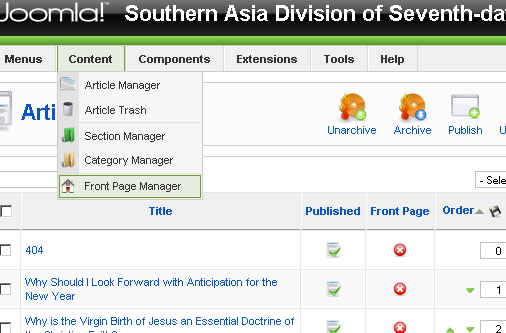
\includegraphics[scale=0.8]{articleFrontPageLink}
\par}

{\selectlanguage{english}
From the article manager, you can add, edit, publish, unpublish, delete,
and perform many other operations on the articles on the website.}

{\selectlanguage{english}
The articles are organized into categories and then the categories
comprise sections. \ For example, the Southern Asia Division News
articles are in the ``Division News'' category which is found in the
``News'' section. \ The Barn articles are found in the ``Barn''
category of the ``Articles'' section. \ The articles in the ``Division
News'' category are the ones that show up when you click on the
``Division News'' item in the main menu on the website. \ Similarly,
the Barn articles are shown when you click on the ``Barn'' item in the
main menu.}

\clearpage\section{}
\subsection[Adding New Articles]{\rmfamily\upshape Adding New Articles}

\bigskip

\liststyleLi
\begin{enumerate}
\item {\selectlanguage{english}
From the article manager, click on the ``New'' button in the upper right
hand corner. }
\end{enumerate}
{\centering\selectlanguage{english}
[Warning: Draw object ignored]
\par}

\liststyleLi
\setcounter{saveenum}{\value{enumi}}
\begin{enumerate}
\setcounter{enumi}{\value{saveenum}}
\item {\selectlanguage{english}
Once on the new article page, fill in the title, section, category,
published, and front page information (it is not necessary to fill in
the alias in since it will be completed automatically).}
\end{enumerate}
{\centering\selectlanguage{english}
[Warning: Draw object ignored]
\par}

\liststyleLi
\setcounter{saveenum}{\value{enumi}}
\begin{enumerate}
\setcounter{enumi}{\value{saveenum}}
\item {\selectlanguage{english}
If you are creating an article for Barn, then select ``Articles'' from
the ``Section'' drop{}-down menu. \ If you are creating an article for
the Southern Asia Division News, then select ``News'' from the
``Section'' drop{}-down menu. \ Either way, the correct category should
automatically be selected in the ``Category'' drop{}-down menu.}
\item {\selectlanguage{english}
If you want the article to show up on the front page of the website then
select ``Yes'' for the ``Front Page'' selection.}
\item {\selectlanguage{english}
If you are creating a new article, you probably will want it to show up
on the website so leave ``Yes'' selected for the ``Published''
selection.}
\item {\selectlanguage{english}
Next you are ready to edit your article using the article text editor.}
\end{enumerate}
{\centering\selectlanguage{english}
 [Warning: Image not found] 
\par}

\liststyleLi
\setcounter{saveenum}{\value{enumi}}
\begin{enumerate}
\setcounter{enumi}{\value{saveenum}}
\item {\selectlanguage{english}
You can type in the content of your article here or you can edit the
article in a separate program (such as Microsoft Word), copy the
content of that document, and paste it here.}
\item {\selectlanguage{english}
There are other parameters and options that you could set, but the only
thing that remains which will need to be filled out is the Meta-data
information. \ This is important because it factors into how the
article will show up in search results. \ To fill in the meta-data,
select ``Metadata information'' from the menu panes on the right side
of the page.}
\end{enumerate}
{\centering\selectlanguage{english}
 [Warning: Image not found] 
\par}

\liststyleLi
\setcounter{saveenum}{\value{enumi}}
\begin{enumerate}
\setcounter{enumi}{\value{saveenum}}
\item {\selectlanguage{english}
The meta data pane should slide down so that you can enter the
Description and Keywords. \ You can fill in the Author if you feel so
inclined and the Robots field if you know what you are doing.}
\end{enumerate}
{\centering\selectlanguage{english}
 [Warning: Image not found] 
\par}

\liststyleLi
\setcounter{saveenum}{\value{enumi}}
\begin{enumerate}
\setcounter{enumi}{\value{saveenum}}
\item {\selectlanguage{english}
The Description field should just include a short description of the
article (I find the first paragraph of an article usually works quite
well). \ The keywords field should include keywords from the article
separated by commas. \ For example, if an article was about how dairy
cows in Nepal were not producing as much milk, the keywords you entered
might be, ``Nepal, dairy, cows, decline, milk, production.''}
\item {\selectlanguage{english}
All that remains now is to save the article.}
\item {\selectlanguage{english}
If you wish to save your changes and stay on the same page, then click
``Apply.'' \ If you wish to save your changes and return to the main
Article Manager page, then click ``Save.''}
\end{enumerate}
{\centering\selectlanguage{english}
 [Warning: Image not found] 
\par}


\bigskip

\subsection{Adding Pictures to an Article}

\bigskip

\liststyleLii
\begin{enumerate}
\item {\selectlanguage{english}\mdseries
If you wish to have a picture embedded in your article you will need to
use the editor on the edit article page to do so.}
\item {\selectlanguage{english}\mdseries
First, click on the ``Insert/Edit Image'' button.}
\end{enumerate}
{\centering\selectlanguage{english}\mdseries
 [Warning: Image not found] 
\par}

\liststyleLii
\setcounter{saveenum}{\value{enumi}}
\begin{enumerate}
\setcounter{enumi}{\value{saveenum}}
\item {\selectlanguage{english}
Then you should get the following dialog screen from which you should
select ``Upload.''}
\end{enumerate}
{\centering\selectlanguage{english}
 [Warning: Image not found] 
\par}

\liststyleLii
\setcounter{saveenum}{\value{enumi}}
\begin{enumerate}
\setcounter{enumi}{\value{saveenum}}
\item {\selectlanguage{english}
From the ``Upload'' dialog box, select ``Add'' and locate the picture
you wish to upload from on your hard drive. \ Select the picture and
click ``Open.''}
\end{enumerate}
{\centering\selectlanguage{english}
 [Warning: Image not found] 
\par}

{\centering\selectlanguage{english}
 [Warning: Image not found] 
\par}

\liststyleLii
\setcounter{saveenum}{\value{enumi}}
\begin{enumerate}
\setcounter{enumi}{\value{saveenum}}
\item {\selectlanguage{english}
Once you have selected the pictures you want to upload, click on the
``Upload'' button.}
\end{enumerate}
{\centering\selectlanguage{english}
 [Warning: Image not found] 
\par}

\liststyleLii
\setcounter{saveenum}{\value{enumi}}
\begin{enumerate}
\setcounter{enumi}{\value{saveenum}}
\item {\selectlanguage{english}
Once you see a green check{}-mark next to the file, click on ``Cancel''
to exit the dialog.}
\end{enumerate}
{\centering\selectlanguage{english}
 [Warning: Image not found] 
\par}

\liststyleLii
\setcounter{saveenum}{\value{enumi}}
\begin{enumerate}
\setcounter{enumi}{\value{saveenum}}
\item {\selectlanguage{english}
The next step is to select the picture from the list of pictures in the
middle of the ``Image Manager.'' Even if it seems to already be
selected, make sure to click on it and check that the ``Properties'' at
the top of the image manager get filled in with the default values.}
\end{enumerate}
{\centering\selectlanguage{english}
 [Warning: Image not found] 
\par}

\liststyleLii
\setcounter{saveenum}{\value{enumi}}
\begin{enumerate}
\setcounter{enumi}{\value{saveenum}}
\item {\selectlanguage{english}
Now it is time to fill in the properties with the values that you want.
\ The URL should be filled in automatically, so you do not need to
worry about that, but there are a couple of things here you will want
to change. \ First of all, set the ``Alternate Text'' field to
something that describes the picture. \ This alternate text will be
what people see if they do not download the image (for whatever reason)
or what blind people will hear if they access the site with a screen
reader. \ If the image is simply decoration and the picture
doesn{\textquotesingle}t really add any meaning, leave the ``Alternate
Text'' field blank.}
\item {\selectlanguage{english}
Next, set the ``Dimensions'' of the picture to something reasonable.
\ The default dimensions are probably too big. \ A good thing to do
here would be to leave ``Proportional'' checked (so that the original
width to height ratio is preserved) and set the first box to something
between 200 and 250 pixels. \ That is generally a good size for an
image in an article.}
\item {\selectlanguage{english}
Finally, you will probably want to set the ``Alignment'' of the image to
either ``Left'' or ``Right'' so that the text of the article will flow
around the image. \ You may also want to set a small ``Margin'' for the
edges of the picture so that the text does not get too close.}
\end{enumerate}
{\centering\selectlanguage{english}
 [Warning: Image not found] 
\par}

\liststyleLii
\setcounter{saveenum}{\value{enumi}}
\begin{enumerate}
\setcounter{enumi}{\value{saveenum}}
\item {\selectlanguage{english}
Now all that you have to do is click ``Insert'' and the picture will be
inserted into your article. \ If you want to make any changes to it
later, simply select the picture and click on the ``Insert/Edit
Picture'' button again.}
\end{enumerate}
{\centering\selectlanguage{english}
 [Warning: Image not found] 
\par}

\clearpage\subsection{}
\subsection{Managing Front Page Articles}

\bigskip

\liststyleLiii
\begin{enumerate}
\item {\selectlanguage{english}
After you{\textquotesingle}ve added an article, if you chose to put it
on the front page, you will find that the new article will appear
before the ``Welcome'' article on the front page of the web site.
\ This is undesirable and we are going to change it. \ First of all,
select ``Front Page Manager'' in the ``Content'' drop{}-down menu.}
\end{enumerate}
{\centering\selectlanguage{english}
 [Warning: Image not found] 
\par}

\liststyleLiii
\setcounter{saveenum}{\value{enumi}}
\begin{enumerate}
\setcounter{enumi}{\value{saveenum}}
\item {\selectlanguage{english}
From the front page manager there are several things that you can do,
including changing the order that articles appear on the front page,
removing articles from the front page, and even changing their
published status. \ We will just focus on changing the ordering of
articles on the front page and removing articles from the front page
entirely.}
\end{enumerate}
\subsubsection{Ordering Articles on the Front Page}

\bigskip

\liststyleLiv
\begin{enumerate}
\item {\selectlanguage{english}
Changing the ordering on the front page is incredibly easy. \ Just click
on the green arrows next to the article you wish to move to change its
order.}
\end{enumerate}
{\centering\selectlanguage{english}
 [Warning: Image not found] 
\par}

\subsubsection{Removing Articles from the Front Page}

\bigskip

\liststyleLiv
\setcounter{saveenum}{\value{enumi}}
\begin{enumerate}
\setcounter{enumi}{\value{saveenum}}
\item {\selectlanguage{english}
Removing Articles from the front page is quite easy, too. \ First,
select the articles that you wish to removed by checking the boxes next
to them.}
\end{enumerate}
{\centering\selectlanguage{english}
 [Warning: Image not found] 
\par}

\liststyleLiv
\setcounter{saveenum}{\value{enumi}}
\begin{enumerate}
\setcounter{enumi}{\value{saveenum}}
\item {\selectlanguage{english}
All you have to do now is click on the ``Remove'' button in the upper
right hand corner of the page.}
\end{enumerate}
{\centering\selectlanguage{english}
 [Warning: Image not found] 
\par}
\end{document}
